\chapter{Data Analysis}
As mentioned before, though of fast flipping and tremendous effort to keep electron beam in exactly
the same conditions (intensity, energy, position and angle on target) through 
opposite helicity states, life is not easy and there is no way to achieve such
a goal, after all, no one can understand completely and control every aspect of
something as complicated as an accelerator. There is always various noise caused
in various parts of the machine, though very small in general sense, they are
large compare to what we want to measure, and actually the largest correction
to PV asymmetry. So we need to remove such noise in the raw asymmetry we measured.

We use the same methods to process both PREX-II and CREX data, therefore we will
talk about only CREX data here.

\begin{table}
    \centering
    \begin{tabular}{c | c c c c }
	\hline
	variable    & quadtets    & minirun	& run	& slug	\\
	\hline	    & 86840789	& 8527	& 1386 & 121 \\
	count	    &	&   &	&   \\
	raw asymmetry ($ppk$)	&   \\
	corrected asymmetry ($ppk$)	&   \\
	\hline
	bpm4aX	\\
	bpm4aY	\\
	bpm4eX	\\
	bpm4eY	\\
	bpm12X	\\
	\hline
    \end{tabular}
    \caption{CREX Data Set}
\end{table}

\begin{table}
    \begin{tabular}{c | c c c}
	\hline
	variable    & regression    & dithering	    & Lagrangian    \\
	\hline
	slope	\\
	correction ($ppm$)  \\
	\hline
    \end{tabular}
\end{table}

CREX started commissioning around December 2019, we took the first good run on 
Dec 12. 6 slugs (slug 100 - 105) were collected before the Christmas. After 
the Christmas break, data taking was resumed until Jan 18 2020 when the \Ca 
target was damaged accidently. It tooks 5 days to prepare a new \Ca target.
Things moving on quite smoothly, we had 2 days of transverse asymmetry 
measurement from Feb 10 to Feb 12. We were a little over halfway on data taking 
when Covid-19 hitted and the lab was shut down at the end of March 2020. Fortunately,
things came back 4 months later, we had the chance to continue data taking for
about 1 month. The experiment stopped data taking on Sep 18 2020. A total charge
of 480 C was collected, among which 390 C was good charge. The dataset was clearly
seperated into 3 parts: before AT, after AT (before Covid) and after Covid, which
we will talk about later.
\begin{figure}[h!]
    \begin{tikzpicture}
	\begin{scope}
	    \node[anchor=south west, inner sep=0] (image) at (0, 0)
	    {   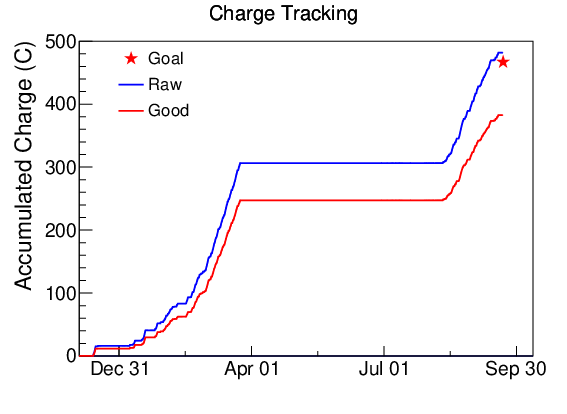
\includegraphics[width=0.45\linewidth]{charge_vs_time}
		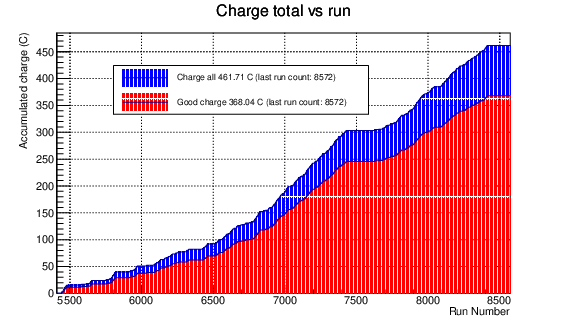
\includegraphics[width=0.54\linewidth]{charge_vs_run} };
	    \begin{scope}[x={(image.south east)},y={(image.north west)}]
		\node [Violet] at (0.27, 0.8) {Covid-shutdown};
		\draw [-stealth, Violet, line width=1pt] (0.28, 0.75) -- (0.28, 0.6);
		\node [Violet] at (0.14, 0.65) {AT};
		\draw [-stealth, Violet, line width=1pt] (0.14, 0.65) -- (0.14, 0.3);
	    \end{scope}
	\end{scope}
    \end{tikzpicture}
    \caption{Charge accumulation versus time (left) and run number (right). The
    long plateau on the left plot is due to Covid shutdown, which is shown around
    run 7500 on the right plot. We see that data taking is most efficient after
    AT (before Covid), the last month (after Covid) is not bad while the 
    first 2 months is not so efficient due to various problems.}
\end{figure}

CREX collected 1451 production runs, among them, 1386 were identified as `Good'
and used for final analysis. The good runs consists of 1362 both arms runs,
6 left arm runs and 18 right arm runs. Each good production run took about $1\ hour$
and collected about $0.3\ C$ charge with a charge efficiency of 80\%.
\begin{figure}[h!]
    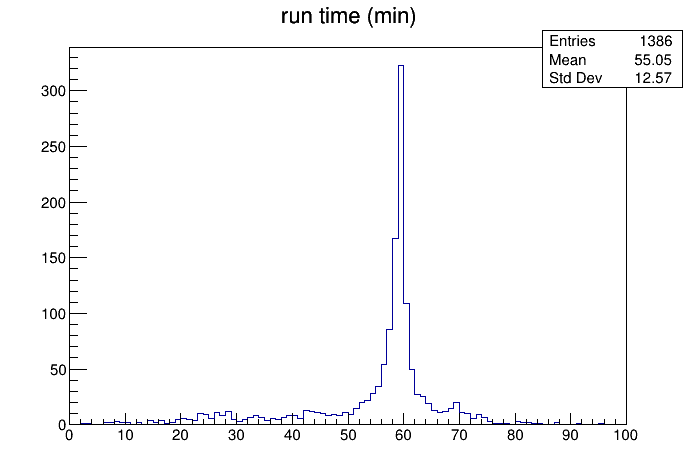
\includegraphics[width=0.32\linewidth]{crex_run_time}
    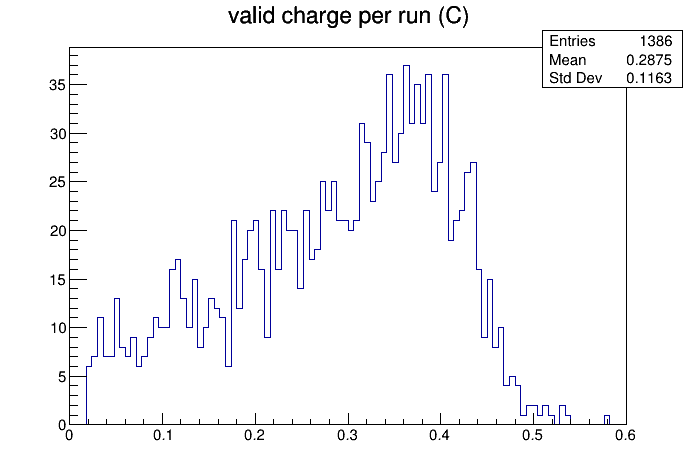
\includegraphics[width=0.32\linewidth]{crex_run_charge}
    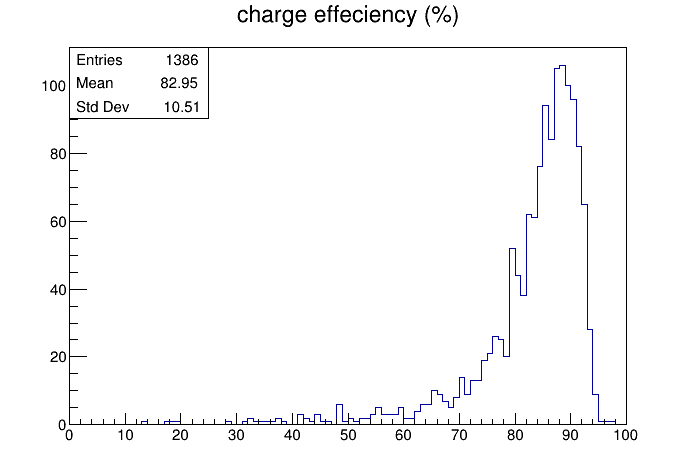
\includegraphics[width=0.32\linewidth]{crex_run_charge_efficiency}
    \caption{Statistics of CREX runs}
\end{figure}

Though electrons come bunch by bunch, the bunch frequency of $249.5\ MHz$ is much
larger than our helicity frequency of $120\ Hz$, so electron beam can be regarded
as continous. All electrons within one helicity window will be integrated as 1
record. Every 4 continuous helicty window data is grouped as quadruplet 
in order to cancel the $60\ Hz$ noise in line power, and asymmetry will be 
calculated based on quadruplet -- this is what we called one asymmetry event.
So the asymmetry event frequency is $30\ Hz$. CREX collects ??? such good 
asymmetry events.

Every run is seperated into multiple miniruns to account for the fact beam
conditions is changing quickly, it is inappropriate to calculate slope values
over a 60 mins run. Minirun will be more proper, the beam conditions, and therefore
the slope value should be more stable during such a shorter time period.  
Every minirun contains 9000 good (pass cut) events (5 mins), the last minirun contains 
whatever number of good events that can't be divided into 2 miniruns. 
CREX has 8543 miniruns from 1386 runs, among them, 16 miniruns are discarded
due to noisy beam conditions that were not caught in the previous 2 respins.
To avoid any respin, these miniruns are simply removed, which counts ??? C.

Runs will be grouped into slugs. One slug is defined as all runs before the next
IHWP flipping. With good beam conditions, we could collect 3 slugs per day, so 
each slug took about 8 hours or longer in case of any accidents. CREX collects
124 slugs, after data clean and combination to remove slugs with only 1 runs, 
121 slugs are kept.

Finnaly, slugs will be grouped into part, with different wien flip status. We
have 3 parts as said before.
\begin{figure}
    \centering
    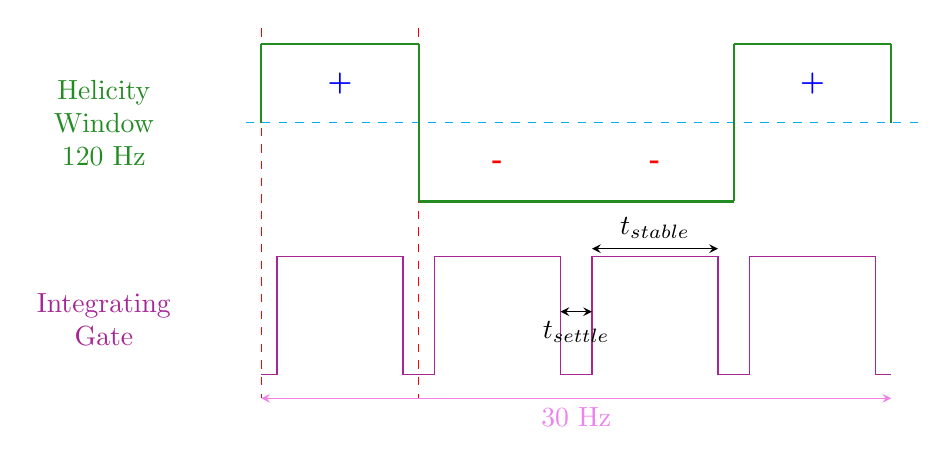
\begin{tikzpicture}[xscale=2]
	\tikzstyle{message} = [align = center]
	\draw[dashed, cyan] (-0.1, 0) -- (4.2, 0);
	\foreach \x in {0, 1}
	{ \draw[dashed, red] (\x, 1.2) -- (\x, -3.5); }
	\foreach \x in {0, 4}
	{ \draw[thick, ForestGreen] (\x, 0) -- (\x, 1); }
	\foreach \x in {1, 3}
	{ \draw[thick, ForestGreen] (\x, -1) -- (\x, 1); }
	\foreach \x in {0, 3}
	{ 
	    \draw[thick, ForestGreen] (\x, 1) -- +(1, 0); 
	    \node[blue] at (\x+0.5, 0.5) {\textbf{+}};
	}
	\foreach \x in {1, 2}
	{ 
	    \draw[thick, ForestGreen] (\x, -1) -- +(1, 0); 
	    \node[red] at (\x+0.5, -0.5) {\textbf{-}};
	}
	\node[message, ForestGreen, very thick] at (-1, 0) {Helicity \\  Window \\ 120 Hz};

	\foreach \x in {0, ..., 3}
	{
	    \draw[Mulberry] (\x, -3.2) -- ++(0.1, 0) -- ++(0, 1.5) -- ++(0.8, 0) 
	    -- ++(0, -1.5) -- ++(0.1, 0);
	}
	\draw[stealth-stealth, black] (2.1, -1.6) -- node[above] {$t_{\text{stable}}$}+(0.8, 0) ;
	\draw[stealth-stealth, black] (1.9, -2.4) -- node[below] {$t_{\text{settle}}$}+(0.2, 0) ;
	\draw[stealth-stealth, Violet] (0, -3.5) -- node[below] {30 Hz} +(4, 0);
	\node[message, Mulberry, very thick] at (-1, -2.5) {Integrating \\ Gate};
    \end{tikzpicture}
    \caption{For CREX, $t_{\text{settle}} = 90\ \mu s$, to allow the PC stablizes
    after flipping, avoiding any cross effect from last helicity state. The 
    deputy factor is 98.92\%.}
\end{figure}

%%%%%%%%%%%%%%%%%%%%%%%%
\subsubsection{Cut}
We have only very loose cut on datas to keep as much data as possible. The online
cuts include a current cut and some stability cuts. The current cut requires
the beam current no smaller than $15\ \mu A$ below the nominal current, due to 
non-linearity in monitor/detector response. The stability cut says ???

a few miniruns are discarded
%%%%%%%%%%%%%%%%%%%%%%%%
\subsubsection{Beam Current}
We have 5 bcms and the upstream analog bcm is used as the target current monitor.
where are the 5 bcms
why choose bcm\_an\_us as bcm\_target?

\begin{itemize}
    \item non-linearity from electronics read out: false asymmetry. PMT $\rightarrow$
	preamplifier $\rightarrow$ ADC
\end{itemize}

Data quality:
\begin{itemize}
    \item Beam excursion: data quality cuts are applied to remove unstable beam periods
	FIXME: a plot for beam excursion
\end{itemize}

%%%%%%%%%%%%%%%%%%%%%%%%%%%%%%%%%%%%%%%%%%%%%%%%%%%%%%%%%%%%%%%%%%%%%%%%
\section{Raw Data}
What we call one event is all electrons counted in one helicity window.
The asymmetry value is calculated using every 4 (8 in PREX-II) helicity windows
(+\-\-+ or -++-)to cancel the 60 Hz line power noise. The helicity pattern was
chosed pseduo-randomly. The CREX data consists of ??? event.

ErrorFlag 

beam jetter ??? in position, ??? in energy and ??? in time scale

Every event
is accompanied by a set of beam parameter values, recording the beam conditions
in that helicity window. A series of cut will be applied, basing on the beam
stability, to select good charge.

\subsubsection{Pair value}
For any 2 continuous events, define their pair value as:
For BPM/BCM, the pair difference is:
$$ diff = \frac{v^+ - v^-}{2} $$

For usl/usr, the asymmetry is:
$$ asym = \frac{v^+ - v^-}{v^+ + v^-} $$

%%%%%%%%%%%%%%%%%%%%%%%%
\subsubsection{Redundant Position Measurement}
stripline BPM vs Cavity BPM

\subsection{Measured Asymmetry}
\subsection{Beam False Asymmetry}

Can we count number of electrons from detector read out?

%%%%%%%%%%%%%%%%%%%%%%%%%%%%%%%%%%%%%%%%%%%%%%%%%%%%%%%%%%%%%%%%%%%%%%%%
\section{Regression}
Regression is the most common statistical method to identify the relationship
between dependent variables (Y) and independent variables (X). Bear in mind that 
regression itself doesn't tell us any relationships or rules, it only works under
the assumption that the relationship of variables is predictable (given by the user) 
and the dependent variables follow a known distribution function $P(\epsilon)$, 
again, needed to be told by the user:
$$ Y = f(X) + \epsilon $$
With these prior knowledge, regression is able to calculate the most likely 
coefficients in the predicted model.

For example, the famous least square fit is actually a linear regression 
$$ Y = c_0 + \sum c_i x_i + \epsilon $$
assuming Gaussian distribution of the dependent variable: $\epsilon \sim N(0, \sigma)$
Another frequenctly used scene is logistic regression for classification, which
is very similar to linear regression except f(X) will be converted into a
probability function, e.x. using the logistic function:
$$ h(z) = \frac{e^z}{1 + e^z} \quad z = f(X) $$

\subsection{The Model}
Considering one monitor and one detector. Assuming the reading noise of detector
follows the Gaussian distribution and the monitor is precise:
\begin{equation*}
    \begin{gathered}
	M = m	\\
	D = d + \epsilon(0, \sigma_0^D)    \\
    \end{gathered}
\end{equation*}
Here, M (D) is the measured value while m (d) is the true value and $\sigma_0^D$ 
is the variance of the noise for Detector.

Then the difference between beams of opposite polarization will follow also
the Gaussian distribution with a larger variance:
\begin{equation*}
    \begin{gathered}
	\Delta M = M^+ - M^- = d^+ - d^-    
	    = \Delta d_0    \\
	\Delta D = D^+ - D^- = (d^+ + \epsilon(0, \sigma_0^D)) - (d^- + \epsilon(0, \sigma_0^D))
	    = \Delta d_0 + \epsilon(0, \sqrt{2}\sigma_0^D)
	    = \Delta d_0 + \epsilon(0, \sigma_1^D) \\
    \end{gathered}
\end{equation*}
Again, $\Delta m_0$ ($\Delta d_0$) is the real difference between the
different polarized beams while $\Delta M$ ($\Delta D$) is the measured value.

The probability for measuring $\Delta D$ will be:
\begin{equation*}
    \begin{gathered}
	P(\Delta D) = \frac{1}{\sigma_1^D\sqrt{2\pi}} e^{-\frac{1}{2}\left( \frac{\Delta D - \Delta d_0}{\sigma_1^D}\right)^2}    \\
    \end{gathered}
\end{equation*}

We will have a bunch of independent data points: $(\Delta M, \Delta D)_i$ and 
we want to extract the relationship between $\Delta d_0$ and $\Delta m_0$: 
$c \equiv \frac{\partial d}{\partial m}$ -- given the tinyness of $\delta m$, first
order is precise enough. This is exactly a linea regression problem.
$$ \Delta d = 0 + c \Delta m $$

For any real data point $(\Delta m_0, \Delta d_0)_i$, the possibility to measure
$(\Delta M, \Delta D)_i$ is:
\begin{equation}
    \begin{gathered}
	P_i(\Delta D|\Delta M) = \frac{1}{\sigma_1^D\sqrt{2\pi}} 
	    e^{-\frac{1}{2}\left( \frac{\Delta D - c\Delta M}{\sigma_1^D}\right)^2}
    \end{gathered}
\end{equation}

For the accumulated data of one minirun, the total probability will be:
\begin{equation}
    P = \prod_i^n P_i(\Delta D|\Delta M) = \prod_i^n \frac{1}{\sigma_1^D\sqrt{2\pi}} 
	    e^{-\frac{1}{2}\left( \frac{\Delta D_i - c\Delta M_i}{\sigma_1^D}\right)^2}
\end{equation}

To maxize P, we have:
\begin{equation}
    \frac{\partial P}{\partial c} = P \times 
    \sum_i \frac{\Delta M_i}{\sigma_1^D} \left( \frac{\Delta D_i - c\Delta M_i}{\sigma_1^D}\right)
    = 0
\end{equation}
Which gives c as:
\begin{equation}
    \sum_i \Delta M_i (\Delta D_i - c\Delta M_i) = 0  \quad \Rightarrow \quad
    c = \frac{\sum \Delta D_i \Delta M_i}{\sum \Delta M^2_i}
\end{equation}

Extend independent variable to multi-dimensional, we have:
\begin{equation}
    \Delta D = \begin{pmatrix} c_1 & c_2 & \cdots & c_n \end{pmatrix} 
	\begin{pmatrix}
	    \Delta M^1	\\
	    \Delta M^2	\\
	    \vdots 	\\
	    \Delta M^n	\\
	\end{pmatrix}
	+ \epsilon(0, \sigma^D)
\end{equation}
\begin{equation}
    \frac{\partial P}{\partial c_\nu} \propto \sum_i \Delta M_i^\nu (\Delta D_i - \sum_\mu c_\mu M_i^\mu) = 0
\end{equation}
Arrange them in a matrix:
\begin{equation}
    \begin{pmatrix}
	\sum_i \Delta D_i \Delta M_i^1 \\
	\sum_i \Delta D_i \Delta M_i^2 \\
	\vdots	\\
	\sum_i \Delta D_i \Delta M_i^n \\
    \end{pmatrix}
    = 
    \begin{pmatrix}
	\sum_i \Delta M_i^1 \Delta M_i^1    & \sum_i \Delta M_i^2 \Delta M_i^1	&
	\cdots	& \sum_i \Delta M_i^n \Delta M_i^1  \\
	\sum_i \Delta M_i^1 \Delta M_i^2    & \sum_i \Delta M_i^2 \Delta M_i^2	&
	\cdots	& \sum_i \Delta M_i^n \Delta M_i^2  \\
	\vdots	& \vdots    & \ddots	& \vdots    \\
	\sum_i \Delta M_i^1 \Delta M_i^n    & \sum_i \Delta M_i^2 \Delta M_i^n	&
	\cdots	& \sum_i \Delta M_i^n \Delta M_i^n  \\
    \end{pmatrix}
    \begin{pmatrix}
	c_1 \\
	c_2 \\
	\vdots	\\
	c_n \\ 
    \end{pmatrix}
\end{equation}

Define covariance of any 2 variables as:
\begin{equation}
    cov(x, y) = \sum_i x_i y_i
\end{equation}

To get:
\begin{equation}
    \begin{pmatrix}
	c_1 \\
	c_2 \\
	\vdots	\\
	c_n \\ 
    \end{pmatrix}
    =
    \begin{pmatrix}
	cov(\Delta M^1, \Delta M^1) & cov(\Delta M^2, \Delta M^1)   & \cdots & cov(\Delta M^n, \Delta M^1)  \\
	cov(\Delta M^1, \Delta M^2) & cov(\Delta M^2, \Delta M^2)   & \cdots & cov(\Delta M^n, \Delta M^2)  \\
	\vdots	& \vdots    & \ddots	& \vdots    \\
	cov(\Delta M^1, \Delta M^n) & cov(\Delta M^2, \Delta M^n)   & \cdots & cov(\Delta M^n, \Delta M^n)  \\
    \end{pmatrix}^{-1}
    \begin{pmatrix}
	cov(\Delta D, \Delta M^1)   \\
	cov(\Delta D, \Delta M^2)   \\
	\vdots	\\
	cov(\Delta D, \Delta M^n)   \\
    \end{pmatrix}
\end{equation}

For multiple detectors, it is easy to get:
\begin{equation}
    \begin{pmatrix}
	c_{11}	& c_{21}    & \cdots & c_{m1}	\\
	c_{12}	& c_{22}    & \cdots & c_{m2}	\\
	\vdots	& \vdots    & \ddots	& \vdots\\
	c_{1n}	& c_{2n}    & \cdots & c_{mn}	\\
    \end{pmatrix}
    =
    \begin{pmatrix}
	cov(\Delta M^1, \Delta M^1) & cov(\Delta M^2, \Delta M^1)   & \cdots & cov(\Delta M^n, \Delta M^1)  \\
	cov(\Delta M^1, \Delta M^2) & cov(\Delta M^2, \Delta M^2)   & \cdots & cov(\Delta M^n, \Delta M^2)  \\
	\vdots	& \vdots    & \ddots	& \vdots    \\
	cov(\Delta M^1, \Delta M^n) & cov(\Delta M^2, \Delta M^n)   & \cdots & cov(\Delta M^n, \Delta M^n)  \\
    \end{pmatrix}^{-1}
    \begin{pmatrix}
	cov(\Delta D^1, \Delta M^1) & cov(\Delta D^2, \Delta M^1)   & \cdots	& cov(\Delta D^m, \Delta M^1)	\\
	cov(\Delta D^1, \Delta M^2) & cov(\Delta D^2, \Delta M^2)   & \cdots	& cov(\Delta D^m, \Delta M^2)	\\
	\vdots	& \vdots    & \ddots	& \vdots    \\
	cov(\Delta D^1, \Delta M^n) & cov(\Delta D^2, \Delta M^n)   & \cdots	& cov(\Delta D^m, \Delta M^n)	\\
    \end{pmatrix}
\end{equation}

Theoretically, we need only 5 BPMs to cover all the beam parameter phase space.
What's the typical noise of bcm/bpm?



%%%%%%%%%%%%%%%%%%%%%%%%%%%%%%%%%%%%%%%%%%%%%%%%%%%%%%%%%%%%%%%%%%%%%%%%
\section{Beam Modulation}

%%%%%%%%%%%%%%%%%%%%%%%%%%%%%%%%%%%%%%%%%%%%%%%%%%%%%%%%%%%%%%%%%%%%%%%%
\section{Lagragian}

%%%%%%%%%%%%%%%%%%%%%%%%%%%%%%%%%%%%%%%%%%%%%%%%%%%%%%%%%%%%%%%%%%%%%%%%
\section{Correction}
\begin{itemize}
    \item background dilution
\end{itemize}
%%%%%%%%%%%%%%%%%%%%%%%%%%%%%%%%%%%%%%%%%%%%%%%%%%%%%%%%%%%%%%%%%%%%%%%%
\section{Result}
